% \usepackage{lineno}
% \begin{linenumbers}
{\actuality} Уравнение состояния (EOS) - описывает фундаментальные свойства ядерной материи, ее эмерджентные макроскопические свойства, обусловленные лежащими в основе сильными взаимодействиями.  
Вблизи плотности насыщения ядерной материи $\rho_{0}$, $\rho_{0}=0.16 фм^{-3}$,  EOS контролирует структуру ядер через энергию связи и несжимаемость $K_{nm}$~\cite{Danielewicz:2002pu}.
EOS также определяет толщину нейтронной оболочки в нейтронно-избыточных ядрах, а также свойства ядерной материи при экстремальных плотностях и/или температурах, соответствующих условиям, возникающим в экспериментах со столкновением релятивистских тяжелых ядер или наблюдаемым в нейтронных звездах  и слияниях нейтронных звезд. 
Более того, исследования показывают, что столкновения тяжелых ионов при энергиях пучка  $E_{kin}$=1.23--10$A$~ГэВ (соответствующих энергиям в системе центра масс $\sqrt{s_{NN}}$ = 2.4--5~ГэВ)  и слияния нейтронных звезд обнаруживают сходные температуры (T $\sim$  50--100~МэВ ) и плотности барионов $\rho \sim (2-5)\rho_{0}$~\cite{Bzdak:2019pkr,Xu:2022mqn}.
Не ограничиваясь описанием свойств материи, состоящей только из протонов и нейтронов, EOS может также отражать появление новых степеней свободы, например, странных частиц в ядрах нейтронных звезд или кварков и глюонов в ультрарелятивистских столкновениях тяжелых ионов. 
Считается, что столкновения ультра-релятивистских тяжелых ионов на Большом адронном коллайдере (LHC) и релятивистском коллайдере тяжелых ионов (RHIC), где  плотность барионов крайне мала, привели к образованию новой формы материи с партонными степенями свободы, обычно называемой сильносвязанной кварк-глюонной материей (КГМ)~\cite{Esumi:2022uas}.
Расчеты квантовой хромодинамики  (КХД) на решетке указывают на то, что при нулевом значении барионного химического потенциала $\mu_{B}$ = 0 и температуре порядка $T \sim  150-160$~МэВ происходит плавный  фазовый переход типа ``кроссовер'' из состояния адронного газа в состояние КГМ. 

В 1955 году Ландау и Беленький~\cite{Belenkij:1955pgn} впервые применили подход вязкой гидродинамики для описания столкновений тяжелых ионов. 
В середине 1970-х годов было выдвинуто предположение что динамика столкновений подвержена влиянию "ударных волн", которые формируются при пересечении сталкивающихся ионов~\cite{Chapline:1973kkq}.
Шилд, Мюллер и Грайнер впервые обратили внимание на значимость расширения области перекрытия в направлении поперечном направлению пучка в работе~\cite{Scheid:1974zz}.
Авторы пришли к заключению, что образованная материя выталкивается перпендикулярно направлению движения сталкивающихся ионов. 
Эффекты коллективного движения частиц проявляются относительно плоскости симметрии, определенной направлением прицельного параметра $b$ и оси пучка $z$.
Эта плоскость получила название плоскости реакции и общепринятое обозначение $\Psi_{RP}$.

Эффект наличия у рожденных в столкновении частиц преимущественного направления вылета впервые был экспериментально обнаружен на установке Plastic Ball/Wall на Линейном ускорителе Беркли~\cite{Gustafsson:1984ka}. 
Ненулевой средний поперечный импульс рожденных частиц направлен в плоскости реакции, перпендикулярно изначальному движению сталкиваемых ионов.
Этот эффект получил название "бокового потока" (sideflow).

Преобладание вылета рожденных частиц перпендикулярно плоскости реакции, вдоль оси $y$ впервые был зафиксирован на эксперименте Diogene в столкновениях с неоновым пучком при энергии $E_{kin}=800A$~МэВ~\cite{Demoulins:1990ac}.
В дальнейшем коллаборация Plastic Ball произвела систематическое исследование этого явления в столкновениях Au~+~Au при различных энергиях~\cite{Gustafsson:1984qh, Gutbrod:1988hh}.

Средний приобретённый импульс рожденных в столкновении частиц может быть охарактеризован наклоном функции в средних быстротах $F=d\langle p_x /A \rangle / dy|_{y=0}$.
В последующие годы экспериментальные измерения среднего импульса были выполнены на множестве экспериментальных установок (EOS, FOPI, E877, E917, E895, NA49 и WA98) в большом диапазоне энергий.
Коллаборация FOPI произвела систематическое исследование направленного и эллиптического потоков для 25 комбинаций систем (Ca+Ca, Ni+Ni, Xe+CsI, Ru+Ru, Zr+Zr, Au+Au) и энергий ($E_{kin}=0.09-1.5A$~ГэВ)~\cite{FOPI:2011aa}. 
На рис.~\ref{fig:Fy_summary} приведена экспериментальная зависимость $F_y$ от энергии столкновения~\cite{Herrmann:1999wu}.
Наблюдается резкое падение коллективного потока с ростом энергии.
Пунктирная линия описывает простое предположение зависимости наклона от времени пролёта сталкивающихся ядер:
%
\begin{equation}
    F(y) = P_{eff} \times S \times t_{pass},
\end{equation}
%
где $P_{eff}$ --- среднее эффективное давление, $S$ --- площадь эффективной расширяющейся поверхности и $t_{pass}$ --- время пролета.
Теоретическое предсказание построено на предположении, что действующая сила $P_{eff} \times S$ постоянна, а уменьшение передачи импульса происходит только из-за сокращения времени пролёта $t_{pass}$.
Эта гипотеза довольно хорошо описывает экспериментальные данные при высоких энергиях, однако не учитывает влияние спектаторов, которое существенно при низких.

\begin{figure}
    \centering
    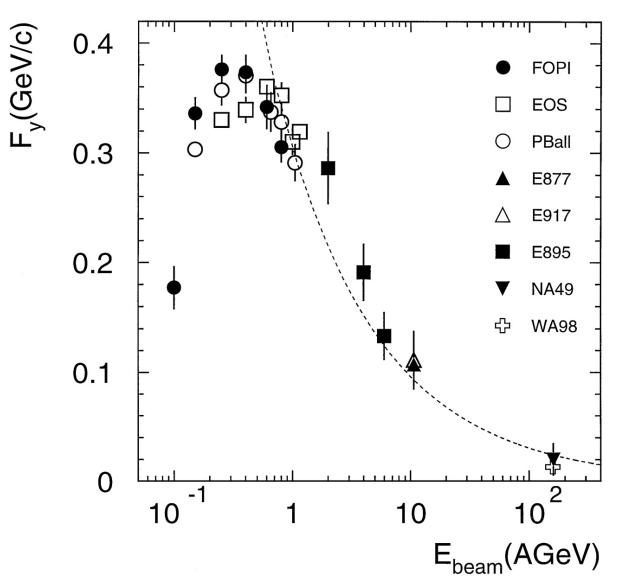
\includegraphics[width=0.55\linewidth]{images/Fy_summary.png}
    \caption{Наклон $F=d\langle p_x /A \rangle / dy|_{y=0}$ как функция энергии столкновения для симметричных систем~\cite{Herrmann:1999wu}.}
    \label{fig:Fy_summary}
\end{figure}

Волошин и Жанг~\cite{Voloshin:1994mz, Poskanzer:1998yz} предложили исследовать импульсную анизотропию рожденных частиц путём разложения азимутального распределения частиц в ряд Фурье:
%
\begin{equation}
    \frac{1}{p_T}\frac{d^3 N}{dp_T dy d\phi} = 
    \frac{ 1 }{2\pi p_T} \frac{ d^2 N }{dp_T dy} \{
    1 + 2\sum_{n=1}^{\infty} v_n(p_T,y) \cos[ n ( \phi - \Psi_R ) ]
    \},
\end{equation}
%
где $\phi$ --- азимутальный угол частицы, $\Psi_{RP}$ --- угол плоскости реакции, определенный вектором прицельного параметра и направлением пучка, $p_T$ --- поперечный импульс и $y$ --- быстрота частицы.
Коэффициенты разложения определяются как 
%
\begin{equation}
    v_n(p_T,y) = \langle  \cos[ n ( \phi - \Psi_R ) ] \rangle,
\end{equation}
%
где угловые скобки означают усреднение по всем частицам и всем событиям. 

На рис.~\ref{fig:v2_energy} показана зависимость эллиптического потока $v_2$ от энергии столкновения для энергий от нескольких МэВ до нескольких ТэВ.
$v_2$ претерпевает две смены знака, начинаясь с положительных значений в области энергий в несколько МэВ на нуклон налетающего ядра. 
Затем очень быстро снижается, достигая минимума в отрицательных значениях, где доминирует эффект "squeeze-out" из-за взаимодействия области перекрытия с остатками сталкивающихся ядер.
С уменьшением времени взаимодействия ($t_pass$) области перекрытия со спектаторами и увеличением энергии столкновения, $v_2$ достигает положительных значений. 
\begin{figure}
    \centering
    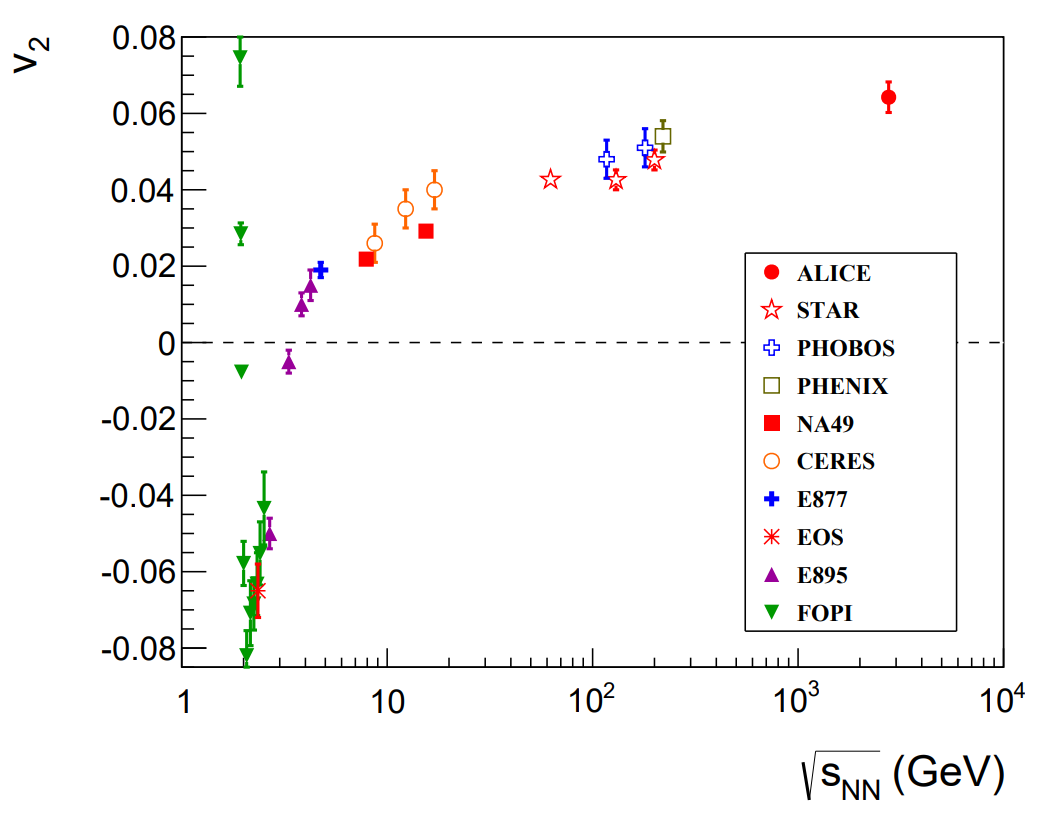
\includegraphics[width=0.5\linewidth]{images/v2_energy.png}
    \caption{Эллиптический поток как функция энергии столкновения~\cite{stock2004relativistic}.}
    \label{fig:v2_energy}
\end{figure}

После открытия КГМ на коллайдере RHIC в 2005 году изучение природы фазового перехода от адронной материи к КГМ и уравнения состояния  квантовой хромодинамики (КХД) в области высоких барионных плотностей стали главной целью программ сканирования по энергии в экспериментах: STAR на коллайдере RHIC ($\sqrt{s_{NN}}$ = 3 - 27~ГэВ), NA61/SHINE на ускорителе  SPS ($\sqrt{s_{NN}}$ = 5.2 - 17~ГэВ)~\cite{NA61:2014lfx}, BM@N на ускорителе Nuclotron ($\sqrt{s_{NN}}$ = 2.3 - 3.5~ГэВ)~\cite{Senger:2022bzm} и   HADES на ускорителе  SIS18 ($\sqrt{s_{NN}}$ = 2.3 - 2.55~ГэВ)~\cite{HADES:2009aat}. 
Строящиеся ускорители FAIR в GSI ($\sqrt{s_{NN}}=3-5$~ГэВ) (Дармштадт) и NICA в ОИЯИ ($\sqrt{s_{NN}}=4-11$~ГэВ) (Дубна) позволят изучить  область высоких барионных плотностей еще более детально.

Транспортные модели описывают распространение частиц в образованной материи при помощи одночастичного потенциала $U(\rho, p)$, где $\rho$ и $p$ --- плотность материи достигнутая в столкновении и импульс частицы.
Этот потенциал часто выражается в виде параметризации Скёрма без импульсной зависимости:
\begin{equation}
    U(\rho) = a(\rho/\rho_0) + b(\rho/\rho_0)^\sigma
    \label{eq:skyrme}
\end{equation}
Параметры $a$, $b$ и $\sigma$ подбираются таким образом, чтобы отвечать свойствам системы: энергия связи на нуклон плотность насыщения и несжимаемость материи K.
Несжимаемость материи в ядерной физике определяется следующим образом:
\begin{equation}
    K = R^2 \frac{d^2 e/\rho}{ d^2 R },
\end{equation}
где вторая производная берётся в предположении постоянного числа нуклонов и энтропии, $e$ --- плотность энергии и $R$ --- радиус ядра.
Предполагается, что коллективное расширение области перекрытия чувствительно к коэффициенту несжимаемости материи $K$.

Сравнение теоретических предсказаний с потенциалом~(\ref{eq:skyrme}) для среднего импульса $\langle p_x / A \rangle$ с экспериментальными данными показывает лучшее согласие для очень больших значений $K \ge 380$~MeV~\cite{Kruse:1985hy, Molitoris:1985gs}.
В то же самое время феноменологический подход с импульсно-зависимым потенциалом, описанный в~\cite{Gale:1987zz, Aichelin:1987ti, Welke:1988zz, Haddad:1995vt} показывает хорошее согласие с данными при относительно небольшой несжимаемости $K=215$~МэВ.
Хотя теоретические модели с импульсно-зависимым потенциалом $U(\rho, p)$ довольно хорошо описывают равновесные свойства ядерной материи, они могут довольно сильно различаться между собой в неравновесной фазе столкновения, которая доминирует в начальные моменты реакции.
Это может влиять на более поздние этапы столкновения и приводить к различной достигнутой плотности.

Благодаря своей чувствительности к деталям начального состояния сильновзаимодействующей материи и ранним временам столкновения, первые два коэффициента разложения Фурье $v_1$ (направленный поток) и $v_2$ (эллиптический поток) являются одними из самих чувствительных к EOS сигналами.
При высоких энергиях столкновения $\sqrt{s_{NN}} > 25$ ГэВ, когда время прохождения сталкивающихся ядер ($t_{pass}<$ 1 фм/c)  меньше типичного времени расширение  материи в области перекрытия ядер ($t_{exp}$), в гармониках потока доминирует коллективное расширение начального распределения партонной плотности. 
Время прохождения $t_{pass}$ зависит от энергии столкновения и размера сталкивающейся системы и его можно оценить как $t_{pass}=2R/y_{beam}$, где R -- радиус ядра и $y_{beam}$ -- быстрота пучка. 
Для столкновений Au+Au при уменьшении энергии столкновения с  $\sqrt{s_{NN}}$=25 ГэВ до 2.4 ГэВ $t_{pass}$ увеличивается с 1 фм/c до 18 фм/c. 
Это увеличивает время взаимодействия рожденных частиц с нуклонами-спектаторами, которые разлетаются преимущественно в плоскости реакции. 
Время расширения материи $t_{exp} \sim R/c_{s}$  определяется ее фундаментальной характеристикой — скоростью звука $c_s$, которая определяет связь  с EOS. 
При энергиях $\sqrt{s_{NN}}$=5--2.4 ГэВ ($E_{kin}$ = 1.23--10$A$~ГэВ) вклад взаимодействия рожденных частиц с нуклонами-спектаторами в наблюдаемые потоки становится значительным. 
Это приводит к росту сигнала направленного потока $v_1$ и уменьшению сигнала эллиптического потока $v_2$ нуклонов с уменьшением энергии столкновения. 
Величина эллиптического потока, а также энергия, при которой $v_2$ меняет знак с положительного на отрицательный, неразрывно связаны с жесткостью EOS ($K_{nm}=9dp/d\rho|_{s/\rho}$): например, более ``жесткий'' EOS приводит как к более быстрому расширению материи в области перекрытия ядер, так и к более сильному блокированию частиц спектаторами, что приводит к большему выдавливанию материи перпендикулярно плоскости реакции  и более отрицательному $v_2$. 
Зависимость направленного потока $v_1(y)$ от быстроты частиц $y$ также чувствительна к EOS, поскольку она измеряет степень отклонения нуклонов-спектаторов в плоскости реакции из-за взаимодействия с материей в области перекрытия. 
Более ``мягкий'' EOS приводит к меньшему отклонению и меньшему наклону  $v_1(y)$ в области средних быстрот. 
Поскольку направленный поток является доминирующим сигналом в области энергий нескольких ГэВ на нуклон и не меняет свой знак, измерения потоков более высоких гармоник часто выполняется относительно плоскости симметрии первого порядка.
Основополагающее ограничение на симметричную часть EOS ядерной материи  в диапазоне плотностей (2-4.5)$\rho_{0}$ было получено путем сравнения измерений, выполненных экспериментом E895 на ускорителе AGS c теоретическими предсказаниями. 
Коллективные потоки  протонов в Au+Au столкновениях при энергиях пучка
$E_{kin}$ = 2--8$A$~ГэВ (соответствующих энергиям  $\sqrt{s_{NN}}$ = 2.7--4.3 ГэВ) сравнивались с результатами моделирования адронного транспорта с использованием EOS с различными значениями несжимаемости $K_{nm}$~\cite{E895:1999ldn,E895:2000maf,E895:2001axb}. 
Попытка извлечь значение коэффициента несжимаемости из данных коллективных потоков была предпринята Данилевичем, Лейси и Линчем в 2002 году~\cite{Danielewicz:2002pu}.
Экспериментальные данные для наклона бокового потока и эллиптического потока были сопоставлены с теоретическими предсказаниями для различных коэффициентов несжимаемости материи $K$.
Сравнение показано на рис.~\ref{fig:Danilewicz}. 
Экспериментальные данные позволили отсечь экстремальные значения коэффициента несжимаемости $K$.

\begin{figure}
    \centering
    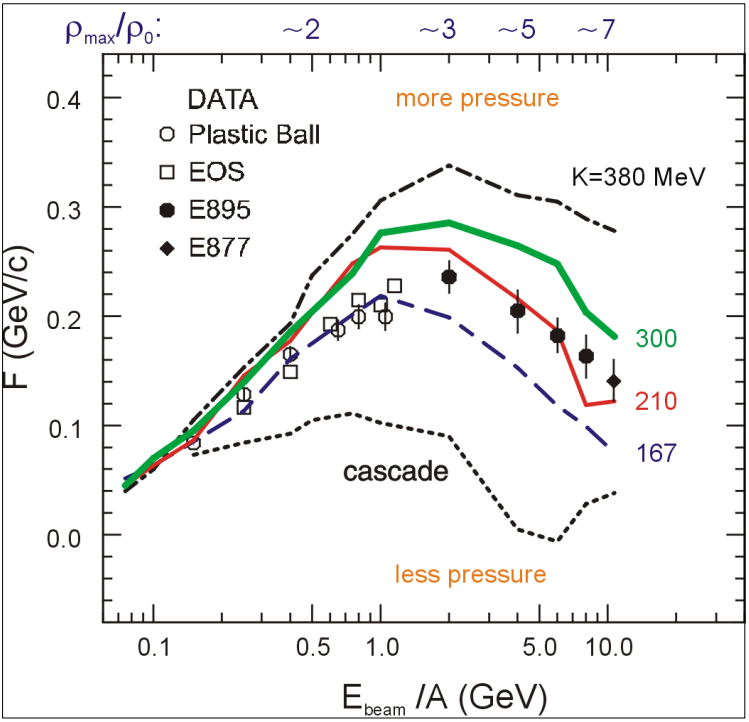
\includegraphics[width=0.45\linewidth]{images/Danilewicz_F_energy.png}
    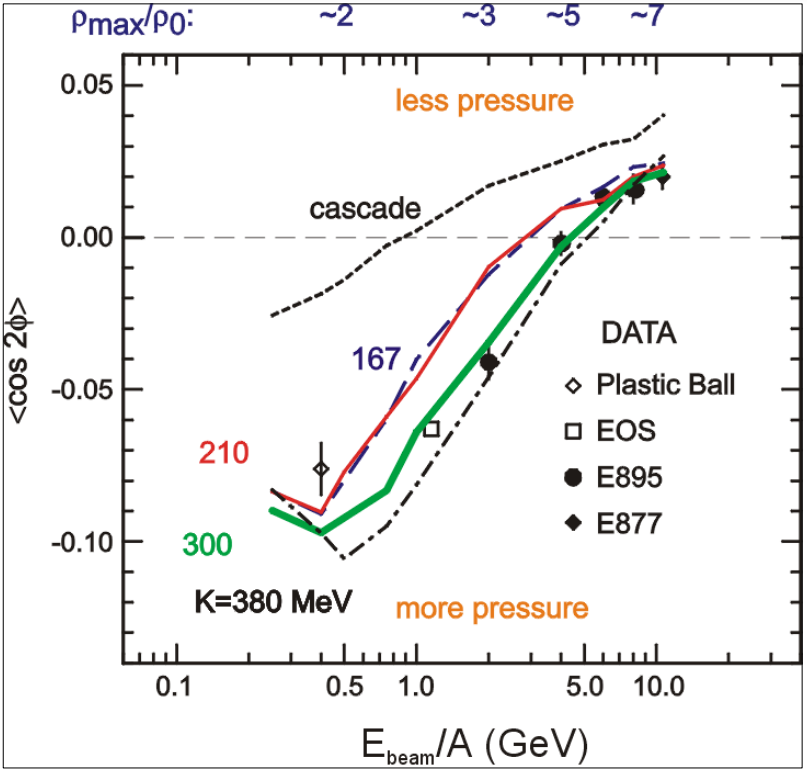
\includegraphics[width=0.45\linewidth]{images/Danilewicz_Elliptic_energy.png}
    \caption{Сравнение данных для наклона бокового потока (слева) и эллиптического потока (справа) как функция энергии с теоретическими расчетами для разных значений коэффициента несжимаемости~\cite{Danielewicz:2002pu}.}
    \label{fig:Danilewicz}
\end{figure}
Однако, интерпретация данных направленного потока $v_1$ протонов требует включения в модель ``мягкого'' EOS с коэффициентом несжимаемости $K_{nm} \sim 210$ МэВ. 
Значения  для эллиптического потока $v_2$ лучше согласуются с более ``жестким'' уравнением состояния $K_{nm} \sim 210$ МэВ~\cite{Danielewicz:2002pu}. 
В дополнение, новые экспериментальные измерения первых двух гармоник коллективных потоков протонов, выполненные экспериментом  STAR на коллайдере RHIC для данных энергий, не согласуются с результатами эксперимента E895.
Одна из причин различия в результатах измерений может заключаться в том, что стандартный метод плоскости событий для измерения анизотропного потока, использовавшийся 15-–20 лет назад экспериментом E895, не учитывал влияние непотоковых корреляций  на измерения $v_n$. 
К непотоковым корреляциям можно отнести следующие эффекты: адронные резонансы и вклад вторичных частиц, сохранение полного(поперечного) импульса, фемтоскопические корреляции. 
Измерение направленного и эллиптического потока в этой области энергий современными методиками подавляющими вклад непотоковых корреляций важны для того чтобы разрешить имеющуюся неоднозначность.
Поэтому высокоточные измерения направленного и эллиптического потока в этой области энергий современными методами анализа подавляющими вклад непотоковых корреляций важны для дальнейшего ограничения значения EOS симметричной сильно-взаимодействующей материи.

В 2017 году эксперимент HADES (High Acceptance Di-Electron Spectrometer)~\cite{HADES:2009aat}, расположенный на ускорителе SIS-18 в GSI, Дармштадт провел набор данных для изучения  столкновений Au+Au  при кинетической энергии пучка $E_{kin}$=1.23$A$~ГэВ ($\sqrt{s_{NN}}$ = 2.4 ГэВ).
В дальнейшем в 2019 году эти измерения были дополнены данными по изучению столкновений Ag+Ag при энергиях пучка $E_{kin}$=1.23 и 1.58$A$ ГэВ.
Это позволило впервые провести высокоточные измерения направленного потока $v_1$ протонов используя современные методики подавляющие вклад непотоковых корреляций.  
Ожидается, что сравнение результатов измерения направленного потока $v_1$ протонов для различных сталкивающихся систем при различных энергиях поможет  оценить вклад взаимодействия рожденных частиц с нуклонами-спектаторами в наблюдаемые коллективные  потоки и получить новые ограничения на значения EOS симметричной материи.
В феврале 2023 года закончился набор данных на первом в России эксперименте по изучению столкновений релятивистских ядер на новом ускорительном комплексе NUCLOTRON-NICA (ОИЯИ, Дубна): "Барионная Материя на Нуклотроне" (BM@N), в ходе которого было набрано порядка 500 М событий столкновений ядер Xe+CsI при кинетической энергии пучка  $E_{kin}$ = 1.23 АГэВ. Данная работа впервые показала возможности измерения коллективных потоков
в эксперименте BM@N,  что значительно расширило его физическую программу по изучению EOS материи  в области высоких барионных плотностей.
Показано, что разработанные и проверенные на экспериментальных данных HADES методики могут быть применены для измерения коллективной анизотропии
рожденных частиц на установке BM@N.

\aim\ представленной работы является экспериментальное исследование коллективной анизотропии протонов,ее рожденных в ядро-ядерных столкновениях  Au + Au и Ag + Ag при энергиях $E_{kin}$=1.23--1.58$A$~ГэВ ($\sqrt{s_{NN}}$=2.4-2.55 ГэВ) на установке HADES (GSI, Дармштадт), а также детальное изучение возможности проведения измерений коллективной анизотропии в эксперименте BM@N на ускорителе NUCLOTRON-NICA (ОИЯИ, Дубна).

Для~достижения поставленной цели необходимо решить следующие {\tasks}:
\begin{enumerate}
    \item  Усовершенствовать  и применить на практике  метод измерения коллективных потоков в экспериментах с фиксированной мишенью с учетом сильной неоднородности азимутального аксептанса установки.

    \item  Разработать метод учета корреляций не связанных с коллективным движением рожденных частиц (непотоковых корреляций) и изучить их влияние на результаты измерения коллективных потоков.

    \item  Исследовать характеристики  направленного потока $v_1$ протонов в столкновениях Au + Au и Ag + Ag при энергиях $E_{kin}$=1.23-1.58$A$~ГэВ ($\sqrt{s_{NN}}$=2.4-2.55 ГэВ) на установке HADES (GSI, Дармштадт).

    \item  Произвести детальное сравнение полученных результатов измерения $v_1$ протонов с теоретическими моделями и данными  других экспериментов.

    \item  Исследовать влияние спектаторов налетающего ядра на формирование $v_1$ протонов с помощью проверки законов масштабирования коллективных потоков с энергией и геометрией столкновения.

    \item  Детально изучить возможности измерения  коллективных потоков протонов на экспериментальной установке BM@N на ускорителе NUCLOTRON-NICA (ОИЯИ, Дубна)
\end{enumerate}

\defpositions
\begin{enumerate}
    \item Зависимости коэффициента направленного потока $v_1$  протонов в зависимости от центральности столкновения, поперечного импульса ($p_T$) и быстроты  ($y_{cm}$) для столкновений Au + Au и Ag + Ag при энергиях $E_{kin}$ =1.23-1.58$A$~ГэВ ($\sqrt{s_{NN}}$=2.4-2.55 ГэВ) на установке HADES (GSI, Дармштадт).
    
    \item Метод учета вклада непотоковых корреляций и изучения их влияния на измеренные значения  коэффициентов потоков $v_n$ для экспериментов с фиксированной мишенью в условиях сильной неоднородности азимутального акспетанса установки.

    \item Результаты сравнения измеренных значений направленного потока ($v_1$) c расчетами в рамках современных моделей ядро-ядерных столкновений, проверка эффекта масштабирования  $v_1$ с энергией столкновения и геометрией области перекрытия.

    \item Исследована эффективность измерения коллективных потоков на экспериментальной установке BM@N на ускорителе NUCLOTRON-NICA (ОИЯИ, Дубна).
\end{enumerate}

\novelty
\begin{enumerate}
    \item Впервые для экспериментов на фиксированной мишени разработаны и апробированы методы коррекции результатов измерения направленного потока на азимутальную неоднородность аксептанса установки и учета корреляций не связанных с  коллективным движением рожденных частиц.

    \item Впервые получены новые экспериментальные измерения направленного потока $v_1$ протонов с учетом вклада непотоковых корреляций для для ядро-ядерных столкновений (Au + Au, Ag + Ag) при энергиях $E_{kin}$ =1.23-1.58$A$~ГэВ ($\sqrt{s_{NN}}$=2.4-2.55 ГэВ), позволяющие оценить вклад нуклонов-спектаторов в коллективную анизотропию частиц.

    \item Методика измерения коллективных анизотропных потоков, опробованная впервые в эксперименте HADES (ГСИ, Дармштадт), была адаптирована к условиям установки BM@N на ускорителе NUCLOTRON-NICA (ОИЯИ, Дубна), и усовершенствована с целью уменьшения систематической ошибки измерения
\end{enumerate}

\influence\ данной работы заключается в том, что коллективная анизотропия рожденных частиц служит одним из главных инструментов исследования уравнения состояния сильно взаимодействующей материи, образованной в области перекрытия сталкивающихся ядер.
Полученные новые прецизионные результаты измерения направленного потока $v_1$ протонов современными методами анализа позволяющими оценить вклад непотоковых корреляций являются принципиально важными для проверки и дальнейшего развития теоретических моделей ядро-ядерных столкновений, получению новых ограничений на значения EOS симметричной сильно-взаимодействующей материи в области максимальной барионной плотности.
Полученный автором работы научно-методический задел лёг в основу программы по измерению коллективных потоков в эксперименте BM@N на ускорителе NUCLOTRON-NICA (ОИЯИ, Дубна). 
Методика измерений была апробирована на основе моделирования детектора BM@N и анализа первых физических данных эксперимента по изучению Xe+Cs(I) столкновений при энергии пучка 3.8 АГэВ.  Данные результаты важны для будущего эксперимента MPD на ускорительном комплексе NICA (ОИЯИ, Дубна), который также может работать в моде эксперимента на фиксированной мишени.

\reliability\ полученных результатов подтверждается их согласованностью с опубликованными данными для измерения  $v_1$ протонов в столкновениях Au + Au при энергии 1.23$A$~ГэВ ($\sqrt{s_{NN}}$=2.4--2.55~ГэВ). Результаты измерения для наклона направленного потока $dv_1/dy|_{y=0}$ в области средних быстрот находятся в хорошем согласии со значениями с других экспериментов (STAR, FOPI)  и следуют зависимости от энергии столкновения и законам масштабирования коллективных потоков в данной области энергий.
Зависимости направленного потока ($v_1$ ) протонов от быстроты и поперечного импульса также согласуются с расчетами Монте-Карло моделей со импульсно-зависимым потенциалом~\cite{nara2019jam}, такими как JAM и UrQMD.
Для разработанных методов измерения коллективных анизотропных потоков была была исследована эффективность их измерений в эксперименте BM@N с помощью Монте-Карло моделирования и последующий полной реконструкции событий.
Хорошее согласие между величинами  $v_n$,  полученными из анализа полностью реконструированных в BM@N частиц  и модельных данных, говорит о высокой эффективности установки для измерения коллективных потоков.

\probation\
Основные результаты работы докладывались~на российских и международных конференциях: Международная конференция «Ядро» (2020, 2021, Россия), Международный Семинар «Исследования возможностей физических установок на FAIR и NICA» (2021, Россия), 
Международная научная конференция молодых учёных и специалистов «AYSS» (2022, 2023, ОИЯИ), Международная конференция по физике элементарных частиц и астрофизике «ICPPA»
(2020, 2022, Россия), Ломоносовская конференция по 
физике элементарных частиц (2023, Россия), XXV Международный Балдинский семинар по проблемам физики высоких энергий (2023, JBZB), 
Международный Семинар «NICA» (2022, 2023, Россия).

\contribution\ Диссертация основана на работах, выполненных автором в рамках международной коллаборации HADES в GSI в 2019-2022~гг и в рамках международной коллаборации BM@N в ОИЯИ в 2022-2024~гг. Из работ, выполненных в соавторстве, в диссертацию включены результаты, полученные лично автором и результаты при его определяющем участии в постановке задач, разработке методов их решения и анализе данных, а также в подготовке результатов измерений для публикации от лица коллабораций HADES и BM@N.
Автор внес определяющий вклад в обработку и анализ экспериментальных данных.
Кроме того, диссертант принимал участие в наборе экспериментальных данных и контроле их качества.

% \publications\ Основные результаты по теме диссертации изложены в 5 печатных работаx, которые опубликованы в переодических научных журналах, входящих в базы данных Web of Science и Scopus.

\ifthenelse{\equal{\thebibliosel}{0}}{% Встроенная реализация с загрузкой файла через движок bibtex8
    \publications\ 
}{% Реализация пакетом biblatex через движок biber
%Сделана отдельная секция, чтобы не отображались в списке цитированных материалов
    \begin{refsection}%
        % \printbibliography[heading=countauthornotvak, env=countauthornotvak, keyword=biblioauthornotvak, section=1]%
        % \printbibliography[heading=countauthorvak, env=countauthorvak, keyword=biblioauthorvak, section=1]%
        % \printbibliography[heading=countauthorconf, env=countauthorconf, keyword=biblioauthorconf, section=1]%
        \printbibliography[heading=countauthor, env=countauthor, keyword=biblioauthor, section=1]%
        \publications\ Основные результаты по теме диссертации изложены в \arabic{citeauthor} статьтях \nocite{Mamaev:2020lpi,Mamaev:2020qom,Mamaev:2023fpr,Mamaev:2023yhz,HADES:2020lob,Mamaev:2024}, которые опубликованы в переодических научных журналах, входящих в базы данных Web of Science и Scopus.
        % \arabic{citeauthorvak} из которых изданы в журналах, рекомендованных ВАК\nocite{vakbib1,vakbib2}, 
        % \arabic{citeauthorconf} "--- в тезисах докладов\nocite{confbib1,confbib2}.
    \end{refsection}
}

% \end{linenumbers}
